\chapter{Evaluation}
\label{chap:evaluation}

The current implementation of SJ supports all the features presented in this paper, including implementations of both the forwarding and resending protocols called \textit{SJFSocket} and \textit{SJRSocket}. This section, first, presents performance measurements for the current SJ runtime implementation, focusing on micro benchmarking of session initiation and the session communication primitives, then I conclude the evaluation of SJ compile and runtime from quality point of view. These preliminary results demonstrate the feasibility of session-based communication and the SJ runtime architecture.

The benchmark applications measure the time to complete a simple two-party interaction: the protocols respectively implemented by the ``Server'' and ``Client'' sides of the interaction are

\begin{equation}
\text{begin}.?[!<\text{MyObject}>]*\text{begin}.~[?(\text{MyObject})]
\end{equation}

which specify that the Server will repeatedly send objects of type \textit{MyObject} for as long as the Client wishes. Full source code is available at \cite{thesis}.

\textit{Socket} serves as the base case (i.e. direct usage of the underlying transport) for comparison with the SJ sockets. For the RMI implementation (RMI), the session iteration is simulated by making consecutive calls to  remote server method with signature $\{\text{MyObject }  \text{getMyObject}(\text{boolean } b)\}$ (the boolean is passed to attain the same communication pattern). Henceforth, a session of length $n$ means that the session-iteration is repeated $n$ times; for RMI, $n$ remote calls.

The benchmark applications measure the time taken for the Client to initiate a session with the Server and finish the session-iteration. For Socket, session initiation simply means establishing a connection to the server. For RMI, the connection is established implicitly by the first remote call (RMI ``reuses'' a server connection for subsequent calls), but we do not include the cost of looking up the remote object in the RMI registry. The RMI dummy run calls an instance of the remote object hosted on the local machine, to avoid creating a connection to the Server before the actual benchmark run.

The benchmarks were conducted using MyObject messages of serialized size 100 Bytes (for reference, an Integer serializes to 81 Bytes) and 10 KBytes for sessions of length 0, 1, 10, 100 and 1000. The results are recorded from repeating each benchmark configuration 1000 times in low (about 0.1ms) and higher latency (about 10ms) environments. RMI was run using the default settings for each platform. 

The low latency environment consisted of two physically neighbouring PCs (Intel Intel Core i5 1.8 GHz, 4 GB RAM) connected via gigabit Ethernet, running Ubuntu 11.04 with Java compiler and runtime (Standard Edition) version 1.7.1. 

\begin{figure}
\centering
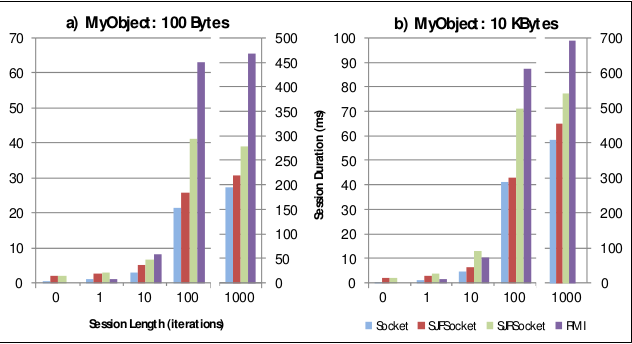
\includegraphics[width=0.8\textwidth]{resources/benchmarking.png}
\caption{Benchmarking}
\label{fig:benchmarking}
\end{figure}

Let first look at the low latency results: The graphs a) and b) in Figure \ref{fig:benchmarking} compare the results from the four benchmark applications over each session length for each of the two MyObject sizes: using pure Socket, SJFSocket, SJRSocket and RMI. The results show that SJFSocket exhibits low runtime overhead in relation to Socket, decreasing for longer sessions. It is important to note that session initiation for both Socket and the session sockets involve establishing a TCP connection, but the SJ sockets do extra work to check session compatibility. SJRSocket is slower than SJFSocket: the cost for session initiation is the same for both, but SJRSocket employs
\begin{compactenum}
\item runtime state tracking and
\item a different routine for serialization and communication.
\end{compactenum}

In fact, comparison of SJFSocket and SJRSocket using sessions that communicate only primitive data types \cite{thesis} show that most of the overhead comes from 2nd item with runtime state tracking incurring little overhead. Despite these additional overheads, SJRSocket performs better than RMI for longer sessions.

The results from the higher latency benchmarks \cite{thesis} also support these observations. We note a few additional points. The cost of session initiation, which involves sending an extra message, increases accordingly. As before, the relative overheads of the SJ sockets become smaller for longer sessions. Indeed, the differences in performance over the longer sessions are minimal.